 \documentclass[10pt,a4paper]{article}
\usepackage{tabularray}
\usepackage{tikz}             
\usepackage{xeCJK}
\usepackage{amsthm}  
\usepackage[fontset=macnew]{ctex}
\usepackage{sgame}
\usepackage{geometry}
\usepackage{amsmath}
\usepackage{amssymb}
\usepackage{graphicx}
\usepackage{sectsty}
\usepackage{color}
\geometry{left=2.cm,right=2.cm,top=3.18cm,bottom=3.18cm}
\usepackage{pgfplots} % package used to implement the plot
\usepackage{pgf-pie}
\usepackage{exscale}
\usepackage{relsize}
\pgfplotsset{width=6.5cm, compat=1.6}
\usepackage{indentfirst}
\usepackage{float}
\usetikzlibrary{shapes,arrows}
\sectionfont{\color{blue}\selectfont}
\subsectionfont{\color{blue}\selectfont}
\subsubsectionfont{\color{blue}\selectfont}
\usepackage{hyperref}
\usepackage{marvosym}
\usepackage{color}
\usepackage{minted}
\usemintedstyle{xcode}
\usepackage{memorygraphs}
\usetikzlibrary{calc,shapes.multipart,chains,arrows.meta}
\usepackage{caption}
\usepackage{makecell}
\newtheorem{definition}{定义}
\newtheorem{theorem}{\textcolor{red}{定理}}
\newtheorem*{solution}{\kaishu 解}
\usepackage[skins]{tcolorbox} %必须标注skin,才能使用shadow命令显示阴影。
\tcbuselibrary{breakable} %breakable:支持跨页
\usepackage{fancyhdr} % 导入fancyhdr包
\pagestyle{fancy}
% 页眉设置
\renewcommand{\familydefault}{\sfdefault}
\usepackage{sansmath} % 导入sansmath宏包
\sansmath
\fancyhead[L]{\textbf{龚舒凯\ 2022202790}}

\begin{document}
	\title{{\Huge 数据结构与算法I实验报告{\large\linebreak\\}}{\huge 实验4:区块链(3)\linebreak\linebreak}}
	\vspace{3cm}
	%\author{\Large 龚舒凯\ 2022202790\ 应用经济-数据科学实验班}
	\author{\\ \Large 龚舒凯\ 2022202790\ 应用经济-数据科学实验班\\
		\hfill\\
		\Large{\url{https://github.com/GONGSHUKAI}}\\
		\hfill}
	
	\date{\today}
	\maketitle
	\newpage
	\begin{center}
		{\huge \textbf{区块链(3):迷你区块链系统}}
	\end{center}
	\section{需求分析}
    \noindent \textbf{问题描述:}在区块链(1)中,我们从文件中读取数据,构造了由一组区块构成的链表。本实验要求在此基础上,实现一个迷你区块链系统,多个节点之间通过“随机”共识来维护一条一致的链,完成消息“收发”处理,以及查询功能。具体而言,该迷你区块链系统中有两个\textbf{区块链节点}和一个\textbf{终端客户节点}:
    \begin{enumerate}
        \item \textbf{区块链节点(server):}每个区块链节点维护一个区块链,除此之外,区块链节点中还有“客户消息队列”和“区块消息队列”,可以根据终端客户发来的客户消息或另一个节点发来的区块消息进行响应,执行交易/查询功能。
        \item \textbf{终端客户(client):}终端客户每隔一定时间随机向另外两个程序发送交易请求或查询请求。交易数据从交易数据集中生成。每条请求将“插入”到对应节点的“客户消息队列”尾部。
    \end{enumerate}

    \noindent \textbf{基本要求:}
    \begin{enumerate}
        \item 多个节点能正常通信,并能维护一个一致的区块链。在两个节点分别按顺序展示链表所有区块,比较是否一致。
        \item 支持按照height或hash查找一个区块;或按照交易id查询一个交易;以及按顺序展示当前链表中所有区块的height和hash值。
    \end{enumerate}
    \noindent \textbf{输出形式:}打开client和server1、server2三个程序,每个程序都有自己的输出,输出内容包括:
    \begin{enumerate}
        \item \textbf{client:}在命令行中输入了客户要求后(transaction或inquiry),显示客户要求的内容,以及消息是否发送成功。
        \item \textbf{server:}如果是客户的交易请求,则显示消息是否处理成功。如果是查询请求,则显示该区块链节点下的查询信息(height/hash/txid)。
    \end{enumerate}
    \begin{figure}[H]
        \centering
            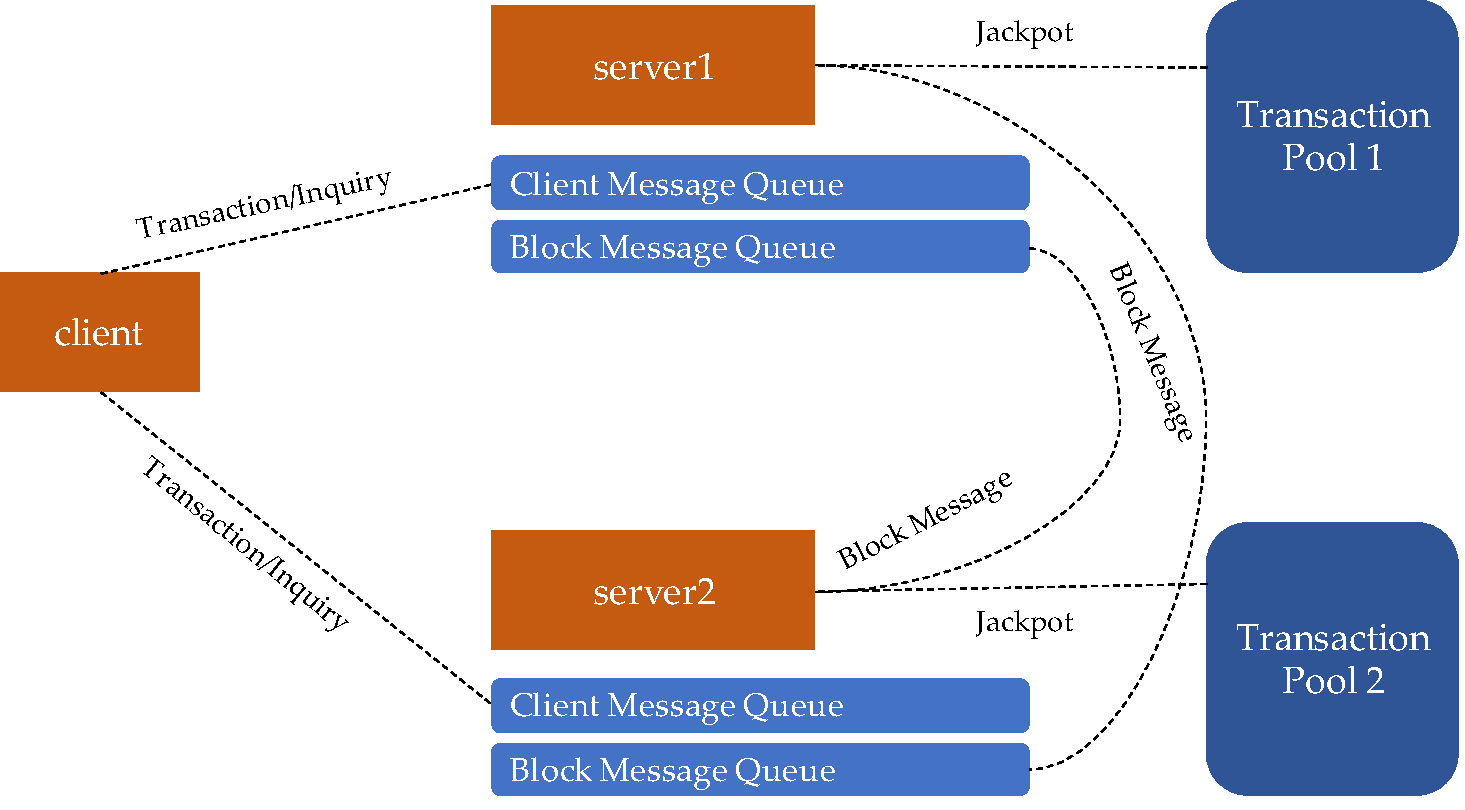
\includegraphics[scale = 0.6]{microBlockChainSystem.pdf}
        \caption{迷你区块链系统示意图}
    \end{figure}
    \newpage
    \section{具体实现}
    \subsection{区块链结构的实现}
    在区块链(1)实验中,我们已经完成了区块链中各组成部分的定义(block, transaction, input, output)、数据集的读取(I/O stream)和按height/txid查找区块/交易的功能。在本实验中,我们将区块链(1)的代码封装为头文件\mintinline{C}|Block_Chain.h|,方便后续在server和client的设计中直接调用。
    \subsection{三个节点的通信}
    在本实验中,通信是通过文件的读写来实现的。每个节点都维护两个文件夹:clientMessage(客户消息)和blockMessage(区块消息)。
    \begin{itemize}
        \item 终端客户向节点$i$发送“客户消息”时,在节点$i$的clientMessage文件夹下写文件“\mintinline{C}|"clientMessage.txt"|,文件内容为客户消息(transaction或inquiry)。
        \item 节点$i$向节点$j$发送“区块消息”时,在节点$j$的blockMessage文件夹下写文件“\mintinline{C}|"blockMessage.txt"|”,文件内容为区块消息(区块链中的一个区块)。
        \item 节点$i$在接受客户消息时,需从自己的clientMessage文件夹下读文件“\mintinline{C}|"clientMessage.txt"|”,将其还原为一个\mintinline{C}|transaction|类型或\mintinline{C}|inquiry|类型的对象。
        \item 节点$i$在接受区块消息时,需从自己的blockMessage文件夹下读文件“\mintinline{C}|"blockMessage.txt"|”,将其还原为一个\mintinline{C}|block|类型的对象。
    \end{itemize}
    终端客户和两个区块链节点的主函数都是无限循环运行的(\mintinline{C}|while(1)|),通过\mintinline{C}|exec|方式同时运行三个程序,并在终端客户处输入指令,即可实现三个节点的通信。\textbf{需要设置三个节点的通信速度上限(例如:间隔5秒发送一条消息),否则会导致磁盘容量溢出。}
    \subsection{终端客户(client)的设计}
    \noindent 终端客户只有两个功能:发送交易请求和发送查询请求:
    \begin{enumerate}
        \item 首先,使用者在终端输入查询类型(是transaction还是inquiry)和查询内容(交易数据集中的交易id或height/hash值)。
        \item 然后,程序用\textbf{随机数生成}的方式随机选取一个节点向其发送消息
    \end{enumerate}
    \noindent 随机数生成调用了\mintinline{C}|#include <random>|,以运行程序的计算机为随机数种子,生成一个服从均匀分布$U[0,1]$的随机数。代码实现如下:
    \begin{minted}[mathescape,linenos,numbersep=5pt,gobble=2,frame=lines,framesep=2mm]{C++}
    int getRandom(int start, int end){
        random_device rd;
        mt19937 gen(rd());
        uniform_int_distribution<> dis(start, end);
        return dis(gen);
    }
    \end{minted}
    \noindent 根据生成的随机数访问对应的区块链节点。\\
    \textbf{如果客户发送的是交易请求,}那么在终端输入要发送的交易的txid。在数据集中找到这一交易后,将交易信息\mintinline{C}|clientMessage1.txt|(数字以此类推)写入区块链节点的\mintinline{C}|clientMessage|文件夹下
    \begin{minted}[mathescape,linenos,numbersep=5pt,gobble=2,frame=lines,framesep=2mm]{C++}
    void sendTransaction(int fileNumber, int server, block *firstblock, block *endblock){
        cout << "Visit Server " << server << endl;
        string fileName = "block_chain_server" + to_string(server) + "/clientMessage/clientMessage" + to_string(fileNumber) + ".txt";
        ofstream outputfile;
        outputfile.open(fileName);
    
        if (outputfile.is_open()){
            string client_txid;
            cout << "Input txid: ";
            cin >> client_txid;
    
            block *p = firstblock;
            int find = 0;//找到交易信息则find = 1, 否则find = 0
            int i = 0;
            int j = 0;
            int k = 0;
            while (p != endblock){
                while (p->transactions[i].txid != ""){
                    if (p->transactions[i].txid == client_txid){
                        outputfile << "Transaction Request" << "\n";
                        outputfile << "transaction" << i << "info"<< "\n";
                        outputfile << p->height << "\n";
                        outputfile << p->transactions[i].txid << "\n";
                        outputfile << p->transactions[i].input_count << "\n";
                        outputfile << p->transactions[i].output_count << "\n";
                        outputfile << p->transactions[i].is_coinbase << "\n";
                        while (p->transactions[i].inputs[j].scriptSig != ""){
                            outputfile << "\n";
                            outputfile << "input" << j << "info"<< "\n";
                            outputfile << p->transactions[i].inputs[j].pre_block << "\n";
                            outputfile << p->transactions[i].inputs[j].prevTxID << "\n";
                            outputfile << p->transactions[i].inputs[j].prevTxOutIndex << "\n";
                            outputfile << p->transactions[i].inputs[j].scriptSig << "\n";
                            j++;
                        }
                        while (p->transactions[i].outputs[k].script != ""){
                            outputfile << "\n";
                            outputfile << "output" << k << "info"<< "\n";
                            outputfile << p->transactions[i].outputs[k].txid << "\n";
                            outputfile << p->transactions[i].outputs[k].index << "\n";
                            outputfile << p->transactions[i].outputs[k].value << "\n";
                            outputfile << p->transactions[i].outputs[k].script << "\n";
                            k++;
                        }                
                        find = 1;//找到这条交易记录
                        break;
                    }
                    i++;
                }
                if (find == 1) break;
                else{
                    i = 0;
                    p = p->next;
                }
            }
            if (find == 1){
                cout << "Message Successfully Sent!" << endl;
                outputfile.close();
            }
            else{
                cout << "Transaction Not Found!" << endl;
            }
        }
        else{
            cout << "Unable to open file";
        }
    }
    \end{minted}
    \noindent \textbf{如果客户发送的是查询请求,}那么在终端输入查询类型(根据height/hash/txid查询),函数调用\mintinline{C}|Block_Chain.cpp|中的查询函数查询区块链节点中的信息。
    \begin{minted}[mathescape,linenos,numbersep=5pt,gobble=2,frame=lines,framesep=2mm]{C++}
    void sendInquiry(int fileNumber, int server, int category, string content){
        cout << "Visit Server " << server << endl;
        string fileName = "block_chain_server" + to_string(server) + "/clientMessage/clientMessage" + to_string(fileNumber) + ".txt";
        ofstream outputfile;
        outputfile.open(fileName);
        if (category == 1){//根据height查询
            outputfile << "height" << "\n";
            outputfile << content << "\n";
            cout << "Message Successfully Sent!" << endl;
            outputfile.close();
        }
        else if (category == 2){//根据hash查询
            outputfile << "hash" << "\n";
            outputfile << content << "\n";
            cout << "Message Successfully Sent!" << endl;
            outputfile.close();
        }
        else{//根据txid查询
            outputfile << "txid" << "\n";
            outputfile << content << "\n";
            cout << "Message Successfully Sent!" << endl;
            outputfile.close();
        }
    }
    \end{minted}
    \subsection{区块链节点(server)的设计}
    \noindent 区块链节点需要完成三大功能
    \begin{enumerate}
        \item 从交易池中抽取交易组成区块并发送区块消息。
        \item 接受区块消息并转化为区块。
        \item 接受客户消息并执行对应的操作,具体而言:
        \begin{enumerate}
            \item 客户消息是交易,则考察是否能将交易加入本区块链节点的交易池。
            \item 客户消息是查询,则从本区块链节点维护的区块链中查询信息。
        \end{enumerate}
    \end{enumerate}
    区块链节点的算法设计可以参考如下伪码:
    \begin{minted}[mathescape,linenos,numbersep=5pt,gobble=2,frame=lines,framesep=2mm]{C++}
    while(1){
        if(中奖){ //中奖调用一个随机数来实现, 中奖几率在0.01-0.1之间
            从“交易池”中取出n (>=1)个交易, 组成一个区块newBLK。
            newBLK的prevHash等于本节点区块链表最后一个区块lastBLK的hash值。
            newBLK的hash值可以采用一个随机函数来生成;
            height值为lastBLK的height+1;
            merkleRoot和nonce都为空。newBLK中的交易集合由上述n个交易构成。
            将newBLK插入本节点的区块链表末尾。
            将newBLK以某个格式组成字符串“发送”给另一个区块链节点的“区块消息队列”。
        }
        else{ //没有中奖
            if(“区块消息队列”不为空){
                从“区块消息队列”头部取出一个消息(内容为区块)
                判断该区块是否与已有区块冲突(即是否存在一个区块, 与新区块的preHash相同。)
                if(冲突) 丢弃该区块;
                else{
                    将该区块插入到本节点区块链表末尾;
                    从“交易池”中删除该区块中包含的交易;
                }
            }
            else{ //“区块消息队列”为空
                从“客户消息队列”头部取出一个消息MSG;
                if(MSG 是交易){
                    if(“交易池”不包含该交易)  将该交易加入“交易池”;
                    else  丢弃该交易;
                }
                else if (MSG 是查询){
                        在本节点维护的区块链表中执行查询;
                        将查询结果输出在屏幕上;
                }
            }
        }
        Sleep(5 seconds);//休眠5秒
    }
    \end{minted}
    两个区块链节点是完全对称的,这里我们只考察区块链节点server1的功能设计。
    \subsubsection{中奖随机数与随机hash生成}
    区块链节点的设计中涉及到两个需要用到随机数/随机字符串生成的地方:分别为\textbf{“中奖”判定}和\textbf{newBLK的hash值生成}。
    
    在这里,我们取中奖概率为0.05,以运行程序的计算机为随机数种子生成一个1到100的均匀分布$U[0,100]$。取到其中5个特定的数判定为“中奖”。随机hash的生成是类似的,我们用一个初始串str来随机生成一个65位的hash字符串。代码实现如下:
    \begin{minted}[mathescape,linenos,numbersep=5pt,gobble=2,frame=lines,framesep=2mm]{C++}
    bool isWinner(){//假设中奖概率为0.05
        random_device rd;
        mt19937 gen(rd());
        uniform_int_distribution<> dis(1, 100);
        vector<int> winningNumbers = {20, 40, 60, 80, 100};
        int randomValue = dis(gen);
        return std::find(winningNumbers.begin(), winningNumbers.end(), randomValue) != winningNumbers.end();
    }
    string randomStringGenerator(){
        string str = "3cc8c69766e26f4ec5b4672e6224cd81c75577674f3cce8c9bb9731a2bb0bd6a";
        random_device rd;
        mt19937 gen(rd());
        uniform_int_distribution<> dis(0, str.length()-1);
        string randomString = "";
        for (int i = 0; i < 64; i++){
            randomString += str[dis(gen)];
        }
        return randomString;
    }
    \end{minted}
    \subsubsection{消息队列的实现}
    区块链节点维护了两个文件夹clientMessage和blockMessage,我们要将其中的客户消息/区块消息按发送时间点的先后整理进入两个队列clientMesageQueue和blockMessageQueue,方便客户消息与区块消息的调取。
    
    遍历文件夹信息需要用到\mintinline{C}|#include <filesystem>|下的\mintinline{C}|filesystem::directory_iterator|类,将文件夹中所有以txt结尾的文件加入队列。需要注意,由于\mintinline{C}|filesystem::directory_iterator|按照文件名的ASCII码从高到低读取文件名,而最先进入文件夹的消息ASCII值是最低的,因此我们需要将读取后的文件名逆序排列,然后加入队列。

    此外,由于文件夹中不断有新的txt文件被写入,而有些未被读取的文件仍滞留在文件夹中。为了不重复将某些消息加入队列,这里设置了一个有序字典\mintinline{C++}|map <string, bool> &processedFiles|用于储存已经入队的文件。在入队列时应检查文件名是否已存在于processedFiles中。
    \begin{minted}[mathescape,linenos,numbersep=5pt,gobble=2,frame=lines,framesep=2mm]{C++}
    queue <string> getTxtFileNames(const string& folderPath, map <string, bool>& processedFiles) {
        queue <string> fileQueue;
        vector<string> sortedFileNames; // 用于存储已排序的文件名
        for (const auto& entry : std::__fs::filesystem::directory_iterator(folderPath)) {
            if (entry.is_regular_file() && entry.path().extension() == ".txt") {
                string fileName = entry.path().filename().string();
                if (processedFiles.find(fileName) == processedFiles.end()) {//如果文件没有进过队列(是写进来的新文件),就将该文件的文件名入队。
                    sortedFileNames.push_back(fileName);
                    //processedFiles[fileName] = true;
                }
            }
        }
        // 对文件名进行排序
        sort(sortedFileNames.begin(), sortedFileNames.end(), [](const string& a, const string& b) {
            return a < b; // 按照ASCII码升序排序
        });
    
        // 将排序后的文件名入队列
        for (const auto& fileName : sortedFileNames) {
            fileQueue.push(fileName);
        }
        return fileQueue;
    }  
    \end{minted}
    
    \subsubsection{区块消息的发送}
    区块链节点的第一大功能是(在“中奖”后)从交易池中抽取交易组成区块并发送区块消息。抽取交易并组成区块的代码实现如下:
    \begin{minted}[mathescape,linenos,numbersep=5pt,gobble=2,frame=lines,framesep=2mm]{C++}
    block* createBlock(block* lastBLK, int n){//从交易池中取出n(>=1)个交易,组成一个区块newBLK。
        block *newBLK = new block;
        newBLK->prevHash = lastBLK->hash;
        newBLK->height = (lastBLK->height) + 1;
        newBLK->merkleRoot = randomStringGenerator();
        newBLK->nonce = 0;
        newBLK->next = NULL;
        newBLK->hash = randomStringGenerator();
    
        vector<transaction> firstNTransactions;//这里就认为取出池中前n个交易
        auto it = transactionPool.begin();
        int count = 0;
        while (it != transactionPool.end() && count < n) {
            firstNTransactions.push_back(it->second);
            ++it;
            ++count;
        }
        for(int i = 0 ; i < n ; i++){
            newBLK->transactions[i] = firstNTransactions[i];
            transactionPool.erase(firstNTransactions[i].txid);//将取出的元素从交易池中删除
        }
        return newBLK;
    }
    \end{minted}
    组成区块后,接下来需将区块信息发送给另一个区块链节点。发送区块的格式如下:
    \begin{itemize}
        \item 先发送区块的基本信息(height, hash, prevHash, merkleRoot, nonce)
        \item 接下来发送区块中每个transaction[i]的信息(txid, input\_count, output\_count, is\_coinbase)
        \item 接下来发送每个transaction下的所有input[j]的信息(prevBlock, prevTxID, prevTxOutIndex, scriptSig)和output[k]的信息(txid, index, value, script)。
    \end{itemize}
    \begin{minted}[mathescape,linenos,numbersep=5pt,gobble=2,frame=lines,framesep=2mm]{C++}
    void sendBlockMessage(int blockMessageNumber, block* newBLK){
        //将newBLK“发送”给另一个区块链节点的“区块消息队列”。
        string fileName = "block_chain_server2/blockMessage/blockMessage" + to_string(blockMessageNumber) + ".txt";
        ofstream outputfile;
        outputfile.open(fileName);
        if (outputfile.is_open()){
            outputfile << newBLK->height << "\n";
            outputfile << newBLK->hash << "\n";
            outputfile << newBLK->prevHash << "\n";
            outputfile << newBLK->merkleRoot << "\n";
            outputfile << newBLK->nonce << "\n";
            int i = 0;
            int j = 0;
            int k = 0;
            outputfile << "\n";
            while (newBLK->transactions[i].txid != ""){
                outputfile << "transaction" << i << "info"<< "\n";
                outputfile << (newBLK->transactions[i]).txid << "\n";
                outputfile << (newBLK->transactions[i]).input_count << "\n";
                outputfile << (newBLK->transactions[i]).output_count << "\n";
                outputfile << (newBLK->transactions[i]).is_coinbase << "\n";
                while (newBLK->transactions[i].inputs[j].scriptSig != ""){
                    outputfile << "\n";
                    outputfile << "input" << j << "info"<< "\n";
                    outputfile << newBLK->transactions[i].inputs[j].pre_block << "\n";
                    outputfile << newBLK->transactions[i].inputs[j].prevTxID << "\n";
                    outputfile << newBLK->transactions[i].inputs[j].prevTxOutIndex << "\n";
                    outputfile << newBLK->transactions[i].inputs[j].scriptSig << "\n";
                    j++;
                }
                while (newBLK->transactions[i].outputs[k].script != ""){
                    outputfile << "\n";
                    outputfile << "output" << k << "info"<< "\n";
                    outputfile << newBLK->transactions[i].outputs[k].txid << "\n";
                    outputfile << newBLK->transactions[i].outputs[k].index << "\n";
                    outputfile << newBLK->transactions[i].outputs[k].value << "\n";
                    outputfile << newBLK->transactions[i].outputs[k].script << "\n";
                    k++;
                }
                i++;
            }
            outputfile.close();
        }
        else{
            cout << "Unable to open file";
        }
    }
    \end{minted}
    \subsubsection{区块消息和交易信息的读取}
    当区块链节点从客户消息队列提取出客户交易请求clientMessage.txt,或从区块消息队列提取出区块信息blockMessage.txt时,需要按照特定的格式将txt转换为transaction类型或block类型的数据结构。依照上文给出的客户消息和区块消息格式,实现还原功能的代码过于冗长,放于附录展出:
    \begin{minted}[mathescape,linenos,numbersep=5pt,gobble=2,frame=lines,framesep=2mm]{C++}
    block* recoverBlock(string fileName);//根据blockMSG.txt文件复原一个block recoverBLK
    transaction recover_tsc(string fileName);//根据clientMSG.txt文件复原一个transaction tsc
    \end{minted}
    \subsubsection{查询功能}
    若终端客户的请求是查询,则在写入区块链节点1的clientMessage文件夹的clientMessage.txt中,第一行显示查询类型(即"height/hash/txid"),于是实现代码为:
    \begin{minted}[mathescape,linenos,numbersep=5pt,gobble=2,frame=lines,framesep=2mm]{C++}
    void inquiryServerBlock(block *serverBlock, string filePath){
        ifstream inputFile(filePath);
        string category;
        string content;
        getline(inputFile, category);// inquiry category: height/hash/txid
        getline(inputFile, content);// inquiry content: heightNumber/hash/txid
        if (category == "height"){
            int heightNumber = stoi(content);
            BlockInfo(heightNumber, serverBlock);
        }
        else if (category == "hash"){
            //Not yet developed :)
        }
        else if (category == "txid"){
            TransactionInfo(content, serverBlock, nullptr);
        }
        else cout << "Wrong inquiry category!" << endl;
    }
    \end{minted}
    \subsubsection{主程序}
    \noindent 依照伪代码描述和上述功能函数,区块链节点的主程序可以写为
    \begin{minted}[mathescape,linenos,numbersep=5pt,gobble=2,frame=lines,framesep=2mm]{C++}
    int main(){
        block *serverBlock = InitServerBlock();
        block *tail = serverBlock;
        int blockMessageNumber = 1;//计数,统计一共发送过几次区块消息,从而给区块消息文件命名
        while(1){
            clientMessageQueue = getTxtFileNames(folderPath1, processedFiles1);
            blockMessageQueue = getTxtFileNames(folderPath2, processedFiles2);
            if (isWinner()){//中奖几率在0.01-0.1之间
                /*从“交易池”中取出n (>=1)个交易,组成一个区块newBLK。
                newBLK的prevHash等于本节点区块链表最后一个区块lastBLK的hash值。
                newBLK的hash值可以采用一个随机函数来生成;
                height值为lastBLK的height+1; merkleRoot和nonce都为空。
                newBLK中的交易集合由上述n个交易构成。
                将newBLK插入本节点的区块链表末尾。
                将newBLK以某个格式(比如JSON)组成字符串“发送”给另一个区块链节点的“区块消息队列”。
                */
                block* newBLK = createBlock(tail, 1);
                tail->next = newBLK;
                tail = newBLK;
                cout << "Jackpot! A new block has been inserted to the chain!" << endl;
                sendBlockMessage(blockMessageNumber, newBLK);
            }
            else{//没有中奖
                if (!blockMessageQueue.empty()){ //“区块消息队列”不为空
                    //从“区块消息队列”头部取出一个消息(内容为区块)
                    //判断该区块是否与已有区块冲突(即是否存在一个区块,与新区块的preHash相同。)
                    string firstBlockMSG = blockMessageQueue.front();//从“区块消息队列”头部取出一个消息(内容为区块)
                    blockMessageQueue.pop();
                    processedFiles2[firstBlockMSG] = true;//将此区块消息标记为被处理过
                    string filePath_BMSG = "block_chain_server1/blockMessage/"+firstBlockMSG;
                    block *firstBLK = recoverBlock(filePath_BMSG);//将该消息恢复成一个区块firstBLK
    
                    if (judgeConflictBlock(firstBLK, serverBlock)){//"冲突"则丢弃该区块
                        cout << "Conflict! The block has been discarded!" << endl;
                    }
                    else{
                    //将该区块插入到本节点区块链表末尾;
                        firstBLK->next = tail->next;
                        tail->next = firstBLK;
                        tail = firstBLK;
                        cout << "The block has been inserted to the chain!" << endl;
                    //从“交易池”中删除该区块中包含的交易;
                        int eraseNum = 0;
                        while (firstBLK->transactions[eraseNum].txid != ""){
                            transactionPool.erase(firstBLK->transactions[eraseNum].txid);
                            eraseNum++;
                        }
                        cout << "Correspondent transactions deleted in the transaction pool!" << endl;
                    }
                }//区块消息队列不为空
                else{//“区块消息队列”为空,从“客户消息队列”头部取出一个消息MSG;
                    if (!clientMessageQueue.empty()){
                        string firstClientMSG = clientMessageQueue.front();//从“客户消息队列”头部取出一个消息MSG;
                        string filePath_CMSG = "/Users/gongshukai/Desktop/SCHOOL WORK/SOPHOMORE SEM1/DATA STRUCTURE  & ALGORITHM /SLIDES & HOMEWORK & LAB/LAB/Oct.27_Lab/block_chain_server1/clientMessage/"+firstClientMSG;
                        clientMessageQueue.pop();
                        processedFiles1[firstClientMSG] = true;//将此客户消息标记为被处理过
                        if (judge_ClientMSG(filePath_CMSG)){//MSG 是交易
                            cout << "Client's transaction request!" << endl;
                            transaction tsc = recover_tsc(filePath_CMSG);
                            if (!find_tsc_in_tscPool(tsc)){//“交易池”不包含该交易,将该交易加入“交易池”;
                                cout << "transaction added to the transaction pool!" << endl;
                                transactionPool.insert(pair<string, transaction>(tsc.txid, tsc));//加入交易池
                            }
                            else{//丢弃该交易
                                cout << "The transaction has been discarded!" << endl;
                            }
                        }
                        else{//MSG 是查询
                            //在本节点维护的区块链表中执行查询;
                            //将查询结果输出在屏幕上;
                            cout << "Client's inquiry request!" << endl;
                            inquiryServerBlock(serverBlock, filePath_CMSG);
                        }
                    }
                }//区块消息队列为空,客户消息队列不为空
            }//中奖or没有中奖
            this_thread::sleep_for(chrono::seconds(5));//隔一会儿再执行下一趟循环,避免server过载
        }//while(1)
    }
    \end{minted}

    \newpage
    \section{使用说明与程序测试样例}
    \subsection{使用说明}
    \subsubsection{终端客户client的使用说明}
    \noindent 首先在终端输入1(代表发送交易请求)或2(代表发送查询请求)
    \begin{enumerate}
        \item 如果输入1(即发送交易请求)
        \begin{enumerate}
            \item 系统随机指定发送到某一区块链节点(server1或server2)
            \item 用户输入要发送的交易txid。注意,txid必须来自于数据集文件,否则无法发送交易。
            \item 终端客户client显示"Message Successfully Sent!",表明已成功向区块链节点发送交易请求。
        \end{enumerate} 
        \item 如果输入2(即发送查询请求)
        \begin{enumerate}
            \item 首先选择查询请求的类型(即根据height/hash/txid查询区块/交易)
            \item 其次输入1或2,代表要查询的区块链节点
            \item 最后输入查询信息,即height/hash/txid
            \item 终端客户client显示"Message Successfully Sent!",表明已成功向区块链节点发送查询请求。
        \end{enumerate}
    \end{enumerate}
    \subsubsection{区块链节点client的显示说明}
    \begin{itemize}
        \item 如果显示"The block has been inserted to the chain!",则表明区块链节点已成功从客户消息队列中提取出另一个区块链节点发送的区块信息,并将其插入本节点维护的区块链末尾。
        \item 如果显示"Conflict! The block has been discarded!",则表明另一节点发送来的区块与本节点区块链中某节点冲突,将该区块丢弃。
        \item 如果显示"Correspondent transactions deleted in the transaction pool!",则表明区块插入本节点区块链末尾后,将该区块中的交易对应的从本节点的交易池中删除。
        \item 如果显示"Client's transaction request!",则表明正在提取客户消息队列的交易请求。 
        \item 如果显示"transaction added to the transaction pool!",则说明交易请求不冲突,已将交易加入到本区块链节点的交易池中。
        \item 如果显示"The transaction has been discarded!",则说明客户发送的交易与交易池中交易冲突,已丢弃该交易。
        \item 如果显示"Jackpot! A new block has been inserted to the chain!",则表明该区块链节点“中奖”,从交易池中提取$n$个交易(本程序中$n=1$)组成一个区块,插入到本区块链末尾的同时也将区块信息发送到另一个区块链节点的区块消息文件夹下。
        \item 如果显示"Client's inquiry request!",则表明正在提取客户消息队列的查询请求。如果接下来终端输出区块信息/交易信息,则说明查询成功。
        \item 如果显示"Block/transaction not found!",则表明客户要查询的区块/交易不存在。
    \end{itemize}
    \subsection{程序测试样例}
    三个程序同时运行的效果如下:
    \begin{figure}[H]
        \centering
            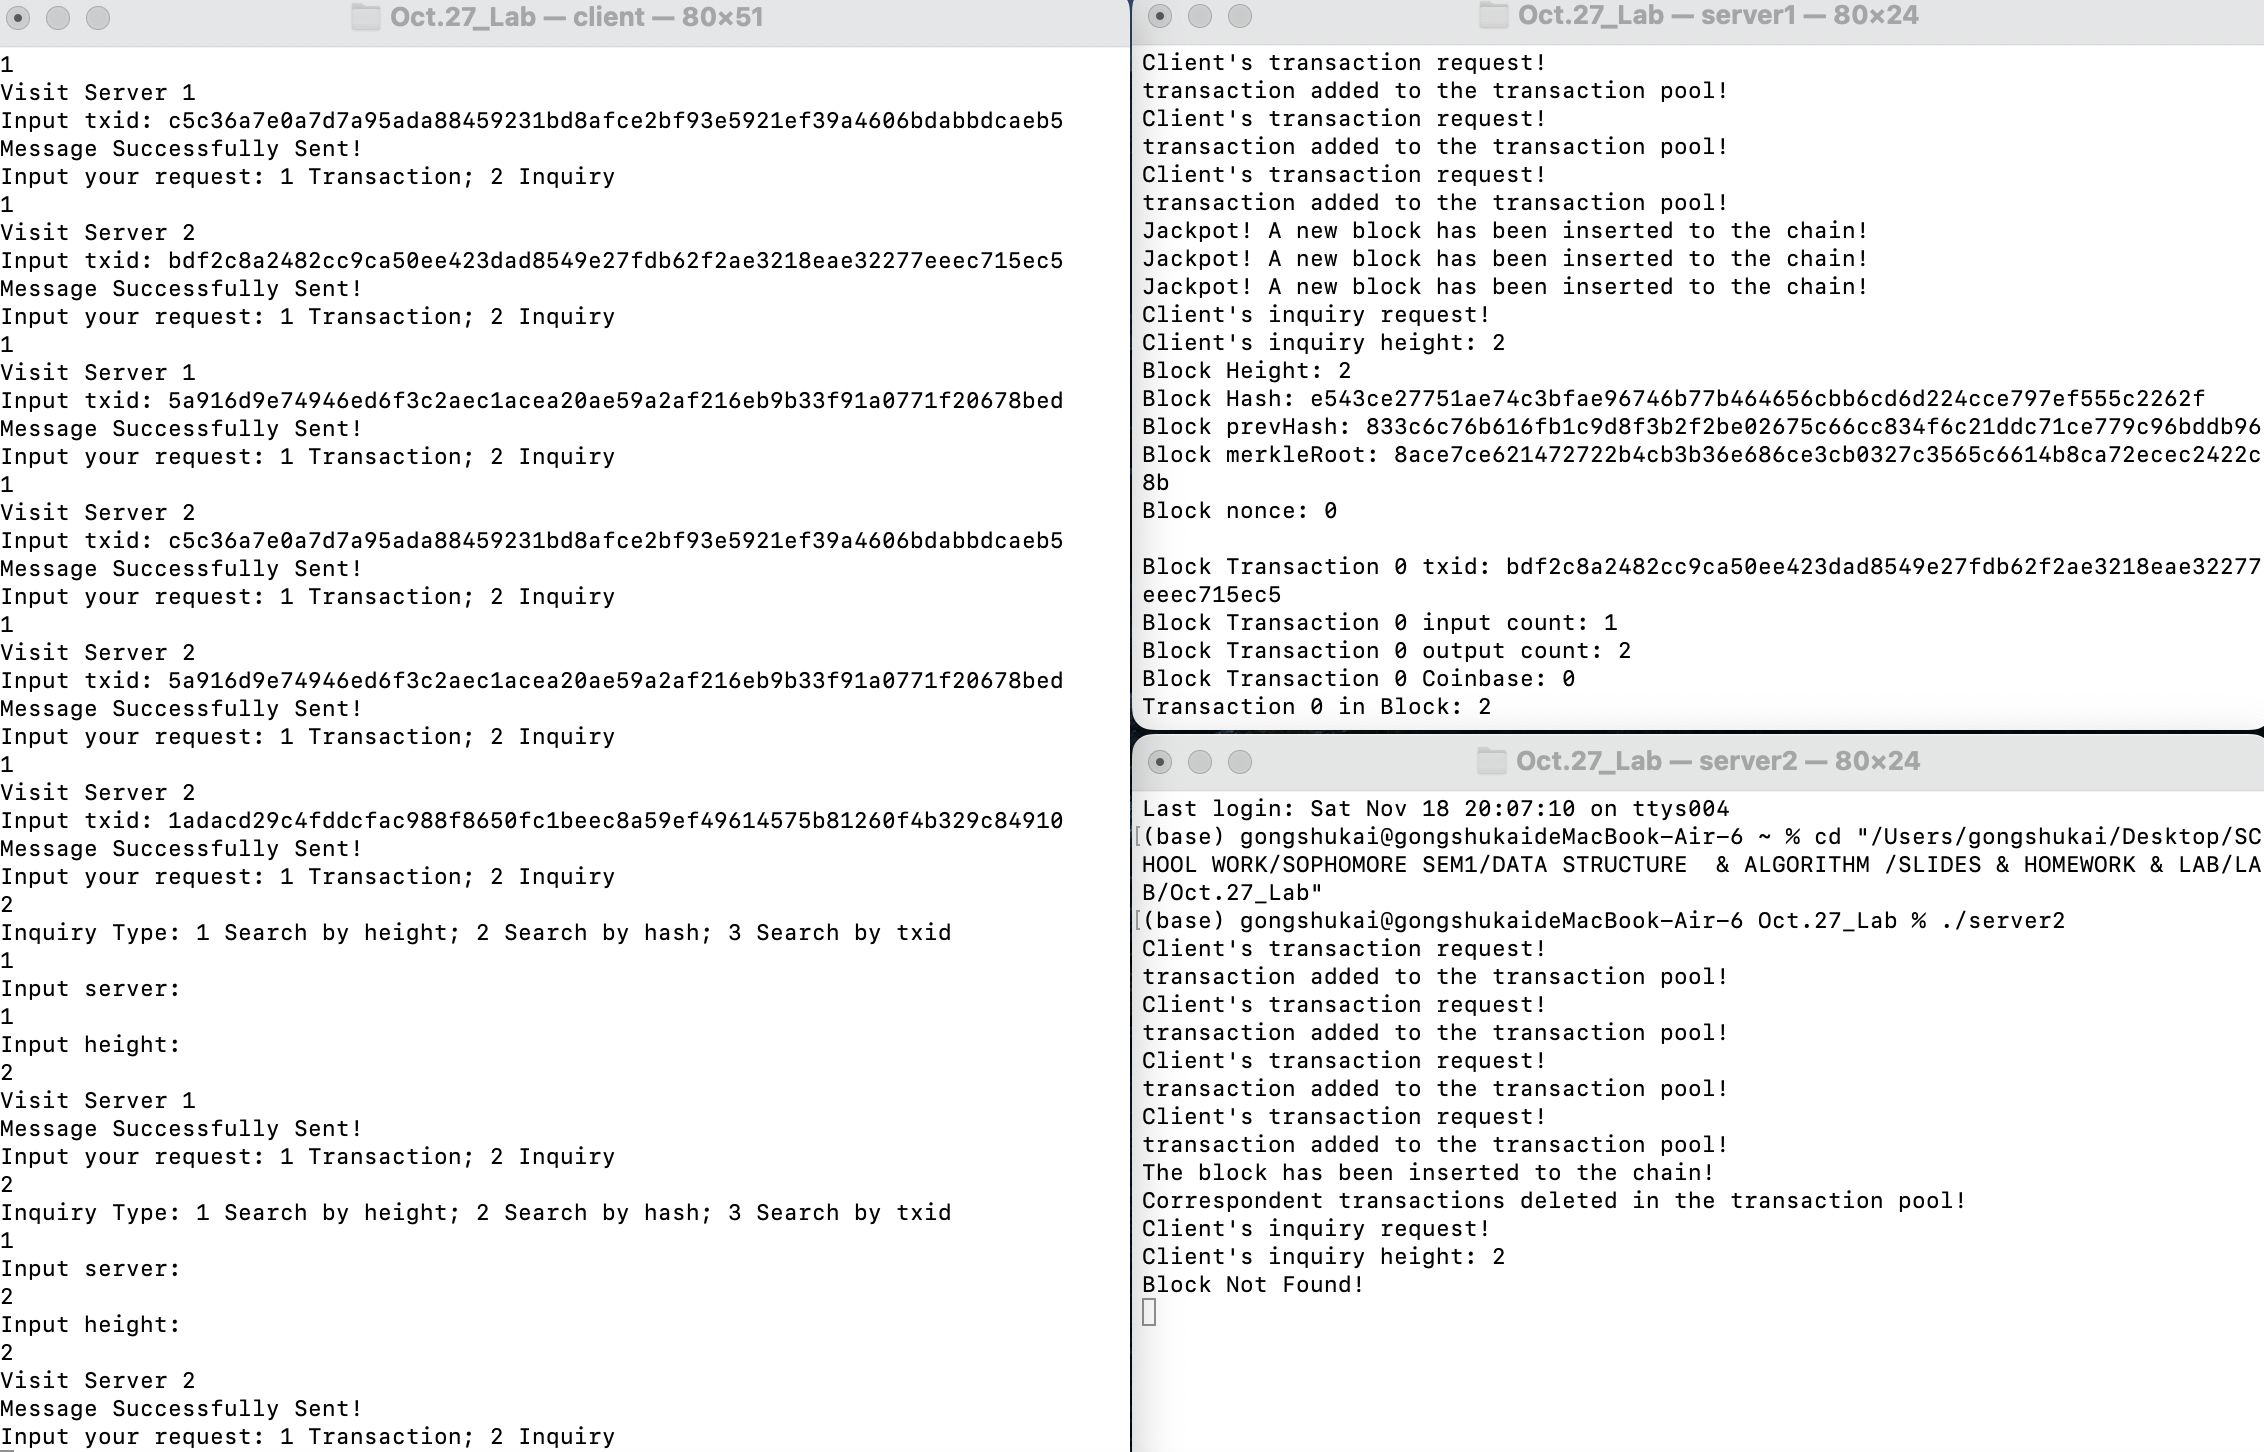
\includegraphics[scale = 0.4]{screenshot.png}
    \end{figure}
\newpage
    \section{附录}
    根目录下所有文件(包括\mintinline{C}|Block_Chain.h|)详见\url{https://github.com/GONGSHUKAI/Data_Structure/tree/main/Lab_Code/Lab_4/Oct.27_Lab},这里展示三个主程序代码\mintinline{C}|client.cpp, server1.cpp, server2.cpp|。\\

    \noindent server1.cpp(server2.cpp的代码是完全相同的,仅根目录代码不同)
    \begin{minted}[mathescape,linenos,numbersep=5pt,gobble=2,frame=lines,framesep=2mm]{C++}
    #include "Block_Chain.h"
    #include <random>
    #include <filesystem>
    #include <map>
    #include <queue>
    #include <chrono>
    #include <thread>
    
    queue <string> clientMessageQueue;//结点1的客户消息队列
    queue <string> blockMessageQueue;//结点1的区块消息队列
    map <string, transaction> transactionPool;//结点1的交易池
    string folderPath1 = "/Users/gongshukai/Desktop/SCHOOL WORK/SOPHOMORE SEM1/DATA STRUCTURE  & ALGORITHM /SLIDES & HOMEWORK & LAB/LAB/Oct.27_Lab/block_chain_server1/clientMessage";//客户消息队列文件夹
    string folderPath2 = "/Users/gongshukai/Desktop/SCHOOL WORK/SOPHOMORE SEM1/DATA STRUCTURE  & ALGORITHM /SLIDES & HOMEWORK & LAB/LAB/Oct.27_Lab/block_chain_server1/blockMessage";//客户消息队列文件夹
    map <string, bool> processedFiles1;//已处理的客户消息队列文件
    map <string, bool> processedFiles2;//已处理的区块消息队列文件
    block* serverBlock;//结点1的区块链
    
    string randomStringGenerator(){
        string str = "3cc8c69766e26f4ec5b4672e6224cd81c75577674f3cce8c9bb9731a2bb0bd6a";
        random_device rd;
        mt19937 gen(rd());
        uniform_int_distribution<> dis(0, str.length()-1);
        string randomString = "";
        for (int i = 0; i < 64; i++){
            randomString += str[dis(gen)];
        }
        return randomString;
    }
    
    bool isWinner(){//假设中奖概率为0.05
        random_device rd;
        mt19937 gen(rd());
        uniform_int_distribution<> dis(1, 100);
        vector<int> winningNumbers = {20, 40, 60, 80, 100};
        int randomValue = dis(gen);
        return std::find(winningNumbers.begin(), winningNumbers.end(), randomValue) != winningNumbers.end();
    }
    
    queue <string> getTxtFileNames(const string& folderPath, map <string, bool>& processedFiles) {
        queue <string> fileQueue;
        vector<string> sortedFileNames; // 用于存储已排序的文件名
        for (const auto& entry : std::__fs::filesystem::directory_iterator(folderPath)) {
            if (entry.is_regular_file() && entry.path().extension() == ".txt") {
                string fileName = entry.path().filename().string();
                if (processedFiles.find(fileName) == processedFiles.end()) {//如果文件没有进过队列(是写进来的新文件),就将该文件的文件名入队。
                    sortedFileNames.push_back(fileName);
                    //processedFiles[fileName] = true;
                }
            }
        }
        // 对文件名进行排序
        sort(sortedFileNames.begin(), sortedFileNames.end(), [](const string& a, const string& b) {
            return a < b; // 按照ASCII码升序排序
        });
    
        // 将排序后的文件名入队列
        for (const auto& fileName : sortedFileNames) {
            fileQueue.push(fileName);
        }
        return fileQueue;
    }
    
    block* InitServerBlock(){
        block* head = new block;
        head->height = 0;//区块高度
        head->hash = "7c5b79677777cc627166cabbc347679b6469749c7cbb7b19617f6c3674c4c3bb";//自定义的头结点的hash
        head->prevHash = "";//前一个区块的哈希值
        head->merkleRoot = "229accb4c760c7c57e7c769e4afce7e434c26757472c281277ceeb36618b2cc5";//本区块中所有交易的默克尔树根
        head->nonce = 114514;//神秘数
        head->next = nullptr;
        return head;//返回节点1的区块链的头结点
    }
    
    block* createBlock(block* lastBLK, int n){//从交易池中取出n(>=1)个交易,组成一个区块newBLK。
        block *newBLK = new block;
        newBLK->prevHash = lastBLK->hash;
        newBLK->height = (lastBLK->height) + 1;
        newBLK->merkleRoot = randomStringGenerator();
        newBLK->nonce = 0;
        newBLK->next = NULL;
        newBLK->hash = randomStringGenerator();
    
        vector<transaction> firstNTransactions;//这里就认为取出池中前n个交易
        auto it = transactionPool.begin();
        int count = 0;
        while (it != transactionPool.end() && count < n) {
            firstNTransactions.push_back(it->second);
            ++it;
            ++count;
        }
        for(int i = 0 ; i < n ; i++){
            newBLK->transactions[i] = firstNTransactions[i];
            transactionPool.erase(firstNTransactions[i].txid);//将取出的元素从交易池中删除
        }
        return newBLK;
    }
    
    void sendBlockMessage(int blockMessageNumber, block* newBLK){
        //将newBLK“发送”给另一个区块链节点的“区块消息队列”。
        string fileName = "/Users/gongshukai/Desktop/SCHOOL WORK/SOPHOMORE SEM1/DATA STRUCTURE  & ALGORITHM /SLIDES & HOMEWORK & LAB/LAB/Oct.27_Lab/block_chain_server2/blockMessage/blockMessage" + to_string(blockMessageNumber) + ".txt";
        ofstream outputfile;
        outputfile.open(fileName);
        if (outputfile.is_open()){
            outputfile << newBLK->height << "\n";
            outputfile << newBLK->hash << "\n";
            outputfile << newBLK->prevHash << "\n";
            outputfile << newBLK->merkleRoot << "\n";
            outputfile << newBLK->nonce << "\n";
            int i = 0;
            int j = 0;
            int k = 0;
            outputfile << "\n";
            while (newBLK->transactions[i].txid != ""){
                outputfile << "transaction" << i << "info"<< "\n";
                outputfile << (newBLK->transactions[i]).txid << "\n";
                outputfile << (newBLK->transactions[i]).input_count << "\n";
                outputfile << (newBLK->transactions[i]).output_count << "\n";
                outputfile << (newBLK->transactions[i]).is_coinbase << "\n";
                while (newBLK->transactions[i].inputs[j].scriptSig != ""){
                    outputfile << "\n";
                    outputfile << "input" << j << "info"<< "\n";
                    outputfile << newBLK->transactions[i].inputs[j].pre_block << "\n";
                    outputfile << newBLK->transactions[i].inputs[j].prevTxID << "\n";
                    outputfile << newBLK->transactions[i].inputs[j].prevTxOutIndex << "\n";
                    outputfile << newBLK->transactions[i].inputs[j].scriptSig << "\n";
                    j++;
                }
                while (newBLK->transactions[i].outputs[k].script != ""){
                    outputfile << "\n";
                    outputfile << "output" << k << "info"<< "\n";
                    outputfile << newBLK->transactions[i].outputs[k].txid << "\n";
                    outputfile << newBLK->transactions[i].outputs[k].index << "\n";
                    outputfile << newBLK->transactions[i].outputs[k].value << "\n";
                    outputfile << newBLK->transactions[i].outputs[k].script << "\n";
                    k++;
                }
                i++;
            }
            outputfile.close();
        }
        else{
            cout << "Unable to open file";
        }
    }
    
    int judge_ClientMSG(string filePath){
        ifstream inputFile(filePath);
        string line;
        getline(inputFile, line);
    
        if (line == "Transaction Request") return 1;//考察ClientMSG.txt的第一行,看他是交易还是查询,是交易则返回true
        else if (line == "") return 2;//文件为空,返回false
        else return 3;
    }
    
    void inquiryServerBlock(block *serverBlock, string filePath){
        ifstream inputFile(filePath);
        string category;
        string content;
        getline(inputFile, category);// inquiry category: height/hash/txid
        getline(inputFile, content);// inquiry content: heightNumber/hash/txid
        if (category == "height"){
            cout << "Client's inquiry height: " << content << endl;//"用户查询的区块高度为:
            int heightNumber = stoi(content);
            BlockInfo(heightNumber, serverBlock);
        }
        else if (category == "hash"){
            cout << "Client's inquiry hash: " << content << endl;
            //Not yet developed :)
        }
        else if (category == "txid"){
            cout << "Client's inquiry txid: " << content << endl;
            TransactionInfo(content, serverBlock, nullptr);
        }
        else cout << "Wrong inquiry category!" << endl;
    }
    
    bool find_tsc_in_tscPool(transaction tsc){
        auto it = transactionPool.find(tsc.txid);
        if (it != transactionPool.end()) return true;//找到了
        else return false;//没找到
    }
    
    bool judgeConflictBlock(block *myBlock, block *serverBlock){
        block *temp = serverBlock;
        while (temp != NULL){
            if (temp->prevHash == myBlock->prevHash) return true;//找到了
            else temp = temp->next;
        }
        return false;//没找到
    }
    
    block* recoverBlock(string fileName) {//根据blockMSG.text文件复原一个block recoverBLK
        block *recoverBLK = new block;
        ifstream inputFile(fileName);
    
        if (inputFile.is_open()) {
            string line;
            unsigned long long transactionIndex = 0;
            unsigned long long inputIndex = 0;
            unsigned long long outputIndex = 0;
    
            // Read block information
            getline(inputFile, line);
            istringstream blockHeight(line);
            blockHeight >> recoverBLK->height;
    
            getline(inputFile, line);
            istringstream blockHash(line);
            blockHash >> recoverBLK->hash;
    
            getline(inputFile, line);
            istringstream blockPrevHash(line);
            blockPrevHash >> recoverBLK->prevHash;
    
            getline(inputFile, line);
            istringstream blockMerkleRoot(line);
            blockMerkleRoot >> recoverBLK->merkleRoot;
    
            getline(inputFile, line);
            istringstream blockNonce(line);
            blockNonce >> recoverBLK->nonce;
    
            recoverBLK->next = nullptr;
            // Skip empty line
            getline(inputFile, line);
    
            while (getline(inputFile, line)) {
                if (line.find("transaction") != string::npos) {
                    // Read transaction information
                    getline(inputFile, line); // Skip transaction info line
                    transaction& tx = recoverBLK->transactions[transactionIndex];
                    istringstream txid(line);
                    txid >> tx.txid;
    
                    getline(inputFile, line);
                    istringstream inputCount(line);
                    inputCount >> tx.input_count;
    
                    getline(inputFile, line);
                    istringstream outputCount(line);
                    outputCount >> tx.output_count;
    
                    getline(inputFile, line);
                    istringstream isCoinbase(line);
                    isCoinbase >> tx.is_coinbase;
    
                    // Read inputs
                    for (int i = 0; i < tx.input_count; i++) {
                        getline(inputFile, line); // Skip empty line
                        getline(inputFile, line); // Skip input info line
                        input& in = tx.inputs[inputIndex];
                        
                        getline(inputFile, line);
                        istringstream pre_block(line);
                        pre_block >> in.pre_block;
                        
                        getline(inputFile, line);
                        istringstream prevTxID(line);
                        prevTxID >> in.prevTxID;
    
                        getline(inputFile, line);
                        istringstream prevTxOutIndex(line);
                        prevTxOutIndex >> in.prevTxOutIndex;
    
                        getline(inputFile, line);
                        istringstream scriptSig(line);
                        ostringstream scriptSigStream;
                        scriptSigStream << scriptSig.rdbuf();  // 将 scriptSig 中的所有字符写入到 ostringstream 中
                        in.scriptSig = scriptSigStream.str();  // 将 ostringstream 中的内容赋值给 in.scriptSig
                        inputIndex++;
                    }
                    // Read outputs
                    for (int i = 0; i < tx.output_count; i++) {
                        getline(inputFile, line);// Skip empty line
    
                        getline(inputFile, line);// Skip output info line
                        output& out = tx.outputs[outputIndex];
    
                        getline(inputFile, line);
                        istringstream txid(line);
                        txid >> out.txid;
    
                        getline(inputFile, line);
                        istringstream index(line);
                        index >> out.index;
    
                        getline(inputFile, line);
                        istringstream value(line);
                        value >> out.value;
    
                        getline(inputFile, line);
                        istringstream script(line);
                        ostringstream scriptStream;
                        scriptStream << script.rdbuf();  // 将 script 中的所有字符写入到 ostringstream 中
                        out.script = scriptStream.str();  // 将 ostringstream 中的内容赋值给 out.script
                        outputIndex++;
                    }
    
                    // Reset input and output index for the next transaction
                    inputIndex = 0;
                    outputIndex = 0;
    
                    // Increment transaction index
                    transactionIndex++;
                }
            }
            inputFile.close();
        }
        return recoverBLK;
    }
    
    transaction recover_tsc(string fileName){
        transaction tx;//根据ClientMSG.txt复原一个transaction tx
        
        ifstream inputFile(fileName);
    
        if (inputFile.is_open()) {
            string line;
            unsigned long long inputIndex = 0;
            unsigned long long outputIndex = 0;
    
            getline(inputFile, line);// Skip transaction request line
    
            // Read transaction information
            getline(inputFile, line); // Skip transaction info line
            getline(inputFile, line); // Skip transaction height
    
            getline(inputFile, line);
            istringstream txid(line);
            txid >> tx.txid;
    
            getline(inputFile, line);
            istringstream inputCount(line);
            inputCount >> tx.input_count;
    
            getline(inputFile, line);
            istringstream outputCount(line);
            outputCount >> tx.output_count;
    
            getline(inputFile, line);
            istringstream isCoinbase(line);
            isCoinbase >> tx.is_coinbase;
    
            // Read inputs
            for (int i = 0; i < tx.input_count; i++) {
                getline(inputFile, line); // Skip empty line
                getline(inputFile, line); // Skip input info line
                input& in = tx.inputs[inputIndex];
                
                getline(inputFile, line);
                istringstream pre_block(line);
                pre_block >> in.pre_block;
                
                getline(inputFile, line);
                istringstream prevTxID(line);
                prevTxID >> in.prevTxID;
    
                getline(inputFile, line);
                istringstream prevTxOutIndex(line);
                prevTxOutIndex >> in.prevTxOutIndex;
    
                getline(inputFile, line);
                istringstream scriptSig(line);
                ostringstream scriptSigStream;
                scriptSigStream << scriptSig.rdbuf();  // 将 scriptSig 中的所有字符写入到 ostringstream 中
                in.scriptSig = scriptSigStream.str();  // 将 ostringstream 中的内容赋值给 in.scriptSig
                inputIndex++;
            }
            // Read outputs
            for (int i = 0; i < tx.output_count; i++) {
                getline(inputFile, line);// Skip empty line
                getline(inputFile, line);// Skip output info line
                output& out = tx.outputs[outputIndex];
    
                getline(inputFile, line);
                istringstream txid(line);
                txid >> out.txid;
    
                getline(inputFile, line);
                istringstream index(line);
                index >> out.index;
    
                getline(inputFile, line);
                istringstream value(line);
                value >> out.value;
    
                getline(inputFile, line);
                istringstream script(line);
                ostringstream scriptStream;
                scriptStream << script.rdbuf();  // 将 script 中的所有字符写入到 ostringstream 中
                out.script = scriptStream.str();  // 将 ostringstream 中的内容赋值给 out.script
                outputIndex++;
            }
            inputFile.close();
        }
        return tx;
    }
    
    
    int main(){
        block *serverBlock = InitServerBlock();
        block *tail = serverBlock;
        int blockMessageNumber = 1;//计数,统计一共发送过几次区块消息,从而给区块消息文件命名
        while(1){
            clientMessageQueue = getTxtFileNames(folderPath1, processedFiles1);
            blockMessageQueue = getTxtFileNames(folderPath2, processedFiles2);
            if (isWinner()){//中奖几率在0.01-0.1之间
                /*从“交易池”中取出n (>=1)个交易,组成一个区块newBLK。
                newBLK的prevHash等于本节点区块链表最后一个区块lastBLK的hash值。
                newBLK的hash值可以采用一个随机函数来生成;
                height值为lastBLK的height+1; merkleRoot和nonce都为空。
                newBLK中的交易集合由上述n个交易构成。
                将newBLK插入本节点的区块链表末尾。
                将newBLK以某个格式(比如JSON)组成字符串“发送”给另一个区块链节点的“区块消息队列”。
                */
                if (transactionPool.empty()){
                    cout << "No transaction in the transaction pool!" << endl;
                    this_thread::sleep_for(chrono::seconds(5));//隔一会儿再执行下一趟循环,避免server过载
                    continue;
                }
                else{
                    block* newBLK = createBlock(tail, 1);
                    tail->next = newBLK;
                    tail = newBLK;
                    cout << "Jackpot! A new block has been inserted to the chain!" << endl;
                    sendBlockMessage(blockMessageNumber, newBLK);
                }
            }
            else{//没有中奖
                if (!blockMessageQueue.empty()){ //“区块消息队列”不为空
                    //从“区块消息队列”头部取出一个消息(内容为区块)
                    //判断该区块是否与已有区块冲突(即是否存在一个区块,与新区块的preHash相同。)
                    string firstBlockMSG = blockMessageQueue.front();//从“区块消息队列”头部取出一个消息(内容为区块)
                    blockMessageQueue.pop();
                    processedFiles2[firstBlockMSG] = true;//将此区块消息标记为被处理过
                    string filePath_BMSG = "block_chain_server1/blockMessage/"+firstBlockMSG;
                    block *firstBLK = recoverBlock(filePath_BMSG);//将该消息恢复成一个区块firstBLK
    
                    if (judgeConflictBlock(firstBLK, serverBlock)){//"冲突"则丢弃该区块
                        cout << "Conflict! The block has been discarded!" << endl;
                        delete firstBLK;
                    }
                    else{
                    //将该区块插入到本节点区块链表末尾;
                        firstBLK->next = tail->next;
                        tail->next = firstBLK;
                        tail = firstBLK;
                        cout << "The block has been inserted to the chain!" << endl;
                    //从“交易池”中删除该区块中包含的交易;
                        int eraseNum = 0;
                        while (firstBLK->transactions[eraseNum].txid != ""){
                            transactionPool.erase(firstBLK->transactions[eraseNum].txid);
                            eraseNum++;
                        }
                        cout << "Correspondent transactions deleted in the transaction pool!" << endl;
                    }
                }//区块消息队列不为空
                else{//“区块消息队列”为空,从“客户消息队列”头部取出一个消息MSG;
                    if (!clientMessageQueue.empty()){
                        string firstClientMSG = clientMessageQueue.front();//从“客户消息队列”头部取出一个消息MSG;
                        string filePath_CMSG = "/Users/gongshukai/Desktop/SCHOOL WORK/SOPHOMORE SEM1/DATA STRUCTURE  & ALGORITHM /SLIDES & HOMEWORK & LAB/LAB/Oct.27_Lab/block_chain_server1/clientMessage/"+firstClientMSG;
                        //如果filePath_CMSG内容为空,执行下一趟循环
                        if (judge_ClientMSG(filePath_CMSG) == 2){
                            this_thread::sleep_for(chrono::seconds(5));//隔一会儿再执行下一趟循环,避免server过载
                            continue;
                        }
                        clientMessageQueue.pop();
                        processedFiles1[firstClientMSG] = true;//将此客户消息标记为被处理过
                        if (judge_ClientMSG(filePath_CMSG) == 1){//MSG 是交易
                            cout << "Client's transaction request!" << endl;
                            transaction tsc = recover_tsc(filePath_CMSG);
                            if (!find_tsc_in_tscPool(tsc)){//“交易池”不包含该交易,将该交易加入“交易池”;
                                cout << "transaction added to the transaction pool!" << endl;
                                transactionPool.insert(pair<string, transaction>(tsc.txid, tsc));//加入交易池
                            }
                            else{//丢弃该交易
                                cout << "The transaction has been discarded!" << endl;
                            }
                        }
                        else if (judge_ClientMSG(filePath_CMSG) == 3){//MSG 是查询
                            //在本节点维护的区块链表中执行查询;
                            //将查询结果输出在屏幕上;
                            cout << "Client's inquiry request!" << endl;
                            inquiryServerBlock(serverBlock, filePath_CMSG);
                        }
                        else{}
                    }
                }//区块消息队列为空,客户消息队列不为空
            }//中奖or没有中奖
            this_thread::sleep_for(chrono::seconds(5));//隔一会儿再执行下一趟循环,避免server过载
        }//while(1)
    }        
    \end{minted}
    
    \noindent client.cpp
    \begin{minted}[mathescape,linenos,numbersep=5pt,gobble=2,frame=lines,framesep=2mm]{C++}
    #include "Block_Chain.h"
    #include <random>
    
    int getRandom(int start, int end){
        random_device rd;
        mt19937 gen(rd());
        uniform_int_distribution<> dis(start, end);
        return dis(gen);
    }
    
    void sendTransaction(int fileNumber, int server, block *firstblock, block *endblock){
        cout << "Visit Server " << server << endl;
        string fileName = "block_chain_server" + to_string(server) + "/clientMessage/clientMessage" + to_string(fileNumber) + ".txt";
        ofstream outputfile;
        outputfile.open(fileName);
    
        if (outputfile.is_open()){
            string client_txid;
            cout << "Input txid: ";
            cin >> client_txid;
    
            block *p = firstblock;
            int find = 0;//找到交易信息则find = 1, 否则find = 0
            int i = 0;
            int j = 0;
            int k = 0;
            while (p != endblock){
                while (p->transactions[i].txid != ""){
                    if (p->transactions[i].txid == client_txid){
                        outputfile << "Transaction Request" << "\n";
                        outputfile << "transaction" << i << "info"<< "\n";
                        outputfile << p->height << "\n";
                        outputfile << p->transactions[i].txid << "\n";
                        outputfile << p->transactions[i].input_count << "\n";
                        outputfile << p->transactions[i].output_count << "\n";
                        outputfile << p->transactions[i].is_coinbase << "\n";
                        while (p->transactions[i].inputs[j].scriptSig != ""){
                            outputfile << "\n";
                            outputfile << "input" << j << "info"<< "\n";
                            outputfile << p->transactions[i].inputs[j].pre_block << "\n";
                            outputfile << p->transactions[i].inputs[j].prevTxID << "\n";
                            outputfile << p->transactions[i].inputs[j].prevTxOutIndex << "\n";
                            outputfile << p->transactions[i].inputs[j].scriptSig << "\n";
                            j++;
                        }
                        while (p->transactions[i].outputs[k].script != ""){
                            outputfile << "\n";
                            outputfile << "output" << k << "info"<< "\n";
                            outputfile << p->transactions[i].outputs[k].txid << "\n";
                            outputfile << p->transactions[i].outputs[k].index << "\n";
                            outputfile << p->transactions[i].outputs[k].value << "\n";
                            outputfile << p->transactions[i].outputs[k].script << "\n";
                            k++;
                        }                
                        find = 1;//找到这条交易记录
                        break;
                    }
                    i++;
                }
                if (find == 1) break;
                else{
                    i = 0;
                    p = p->next;
                }
            }
            if (find == 1){
                cout << "Message Successfully Sent!" << endl;
                outputfile.close();
            }
            else{
                cout << "Transaction Not Found!" << endl;
            }
        }
        else{
            cout << "Unable to open file";
        }
    }
    
    void sendInquiry(int fileNumber, int server, int category, string content){
        cout << "Visit Server " << server << endl;
        string fileName = "block_chain_server" + to_string(server) + "/clientMessage/clientMessage" + to_string(fileNumber) + ".txt";
        ofstream outputfile;
        outputfile.open(fileName);
        if (category == 1){//根据height查询
            outputfile << "height" << "\n";
            outputfile << content << "\n";
            cout << "Message Successfully Sent!" << endl;
            outputfile.close();
        }
        else if (category == 2){//根据hash查询
            outputfile << "hash" << "\n";
            outputfile << content << "\n";
            cout << "Message Successfully Sent!" << endl;
            outputfile.close();
        }
        else{//根据txid查询
            outputfile << "txid" << "\n";
            outputfile << content << "\n";
            cout << "Message Successfully Sent!" << endl;
            outputfile.close();
        }
    }
    
    int main(){
        int request = 0;
        int request2 = 0;
        int fileNumber1 = 1;
        int fileNumber2 = 1;
        block* firstBlock = InitBlockChain();
        while(1){
            cout << "Input your request: 1 Transaction; 2 Inquiry" << endl;
            cin >> request;
            if (request == 1){
                int server = getRandom(1, 2);
                if (server == 1){
                    sendTransaction(fileNumber1, 1, firstBlock, nullptr);
                    fileNumber1++;
                }
                else{
                    sendTransaction(fileNumber2, 2, firstBlock, nullptr);
                    fileNumber2++;
                }
            }
            else if (request == 2){
                cout << "Inquiry Type: 1 Search by height; 2 Search by hash; 3 Search by txid" << endl;
                cin >> request2;
                if (request2 == 1){//按照height查询
                    cout << "Input server: " << endl;
                    int server;
                    cin >> server;
                    string height;
                    cout << "Input height: " << endl;
                    cin >> height;
                    if (server == 1){
                        sendInquiry(fileNumber1, server, 1, height);
                        fileNumber1++;
                    }
                    else{
                        sendInquiry(fileNumber2, server, 1, height);
                        fileNumber2++;
                    }
                }
                else if (request2 == 2){//按照hash查询
                    cout << "Input server: " << endl;
                    int server;
                    cin >> server;
                    string hash;
                    cout << "Input hash: " << endl;
                    cin >> hash;
    
                    if (server == 1){
                        sendInquiry(fileNumber1, server, 2, hash);
                        fileNumber1++;
                    }
                    else{
                        sendInquiry(fileNumber2, server, 2, hash);
                        fileNumber2++;
                    }
                }
                else{//按照txid查询
                    cout << "Input server: " << endl;
                    int server;
                    cin >> server;
                    string txid;
                    cout << "Input txid: " << endl;
                    cin >> txid;
                    
                    if (server == 1){
                        sendInquiry(fileNumber1, server, 3, txid);
                        fileNumber1++;
                    }
                    else{
                        sendInquiry(fileNumber2, server, 3, txid);
                        fileNumber2++;
                    }
                }
            }
            else{
                cout << "Invalid Request! Please input again!" << endl;
            }
        }
    }
    \end{minted}
\end{document}
